\section{Geodetic Coordinate System}\label{sec:coord}

\begin{figure}[H]
   \centering
    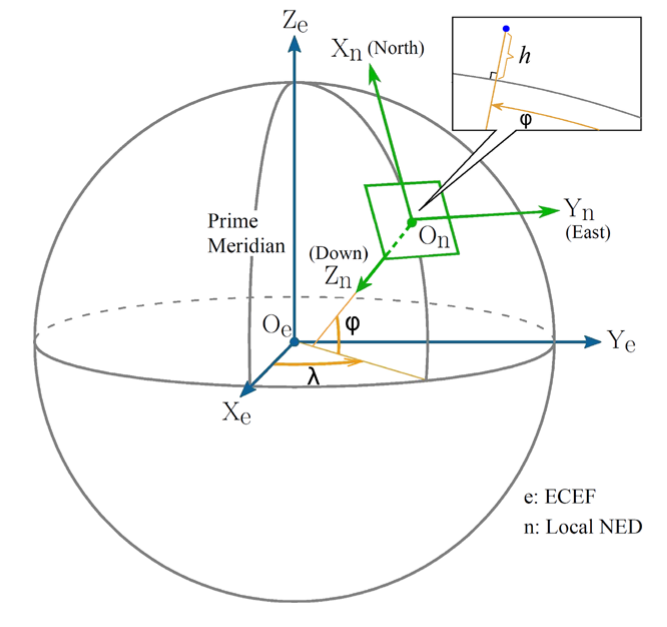
\includegraphics[width=.70\textwidth]{figures/GeoTemp1.png} 
    \label{fig:Geodetic}
    \caption{Geodetic, ECEF and local NED Frames.}  
\end{figure}

\paragraph{}The geodetic coordinate system is widely used in GPS-based navigation. Note that it is not an usual Cartesian coordinate system but a system that
characterizes a coordinate point near the earth’s surface in terms of longitude, latitude, and altitude (or height), which are respectively denoted by $\lambda$, $\varphi$, and h (yellow lines) in figure \ref{fig:Geodetic}.

\paragraph{}The \textit{World Geodetic System} is a standard used in cartography, geodesy and navigation. This standard sets reference points based on an ellipsoidal model of the earth and a gravitational equipotential surface that defines the nominal sea level. Its latest version is \textbf{WGS84}, and that is the one used throughout this project. 

The longitude measures the rotational angle (ranging from $-180$ to $180$ degrees) between the Prime Meridian and the measured point. The latitude measures the angle (ranging from $-90$ to $90$ degrees) between the equatorial plane and the normal of the reference ellipsoid that passes through the measured point. The height (or altitude) is the local vertical distance between the measured point and the reference ellipsoid.

\paragraph{}Thanks to the \textbf{WGS84} standard a list of parameters can be defined that will help us transform the Geodetic Frame to other Coordinate systems:

\begin{align*}
& R_{Ea} = 6,378,137.0 m \\
& f = 1/298.257223563 \\
& R_{Eb} = R_{Ea}(1-f) = 6356752.0m \\
& e = \frac{\sqrt{R_{Ea}^2-R_{Eb}^2}}{R_{Ea}} = 0.08181919 \\
% & M_{E} = \frac{R_{Ea}(1-e^2)}{(1-e^2\sin^2\varphi)^{\frac{3}{2}}}}
\label{eq:los_distToHorizon}
\end{align*} 

\begin{itemize}
\item{Semi-major axis, $R_{Ea}$}
\item{Flattening factor, $f$}
\item{Semi-minor axis, $R_{Eb}$}
\item{First Eccentricity, $e$}
\item{Meridian radius of curvature, $M_{E}$}
\item{Prime vertical radius of curvature, $N_{e}$}
\end{itemize}
